\documentclass[hidelinks]{article}
\usepackage[a4paper, total={7in, 10in}]{geometry}
\usepackage[dvipsnames]{xcolor}
\usepackage{amsmath}
\usepackage{tikz}
\usepackage{tkz-euclide}
\usepackage[unicode]{hyperref}
\usepackage[all]{hypcap}
\usepackage{fancyhdr}
\usepackage[UTF8,fontset=fandol]{ctex}

\usetikzlibrary{angles,calc, decorations.pathreplacing}

\definecolor{carminered}{rgb}{1.0, 0.0, 0.22}
\definecolor{capri}{rgb}{0.0, 0.75, 1.0}
\definecolor{brightlavender}{rgb}{0.75, 0.58, 0.89}

\title{\textbf{Project 1: Solar Eclipse Prediction}}
\author{刘任达\\文哲\\蒋弘杰}
\date{March 24th, 2025}
\begin{document}
\hypersetup{bookmarksnumbered=true,}
\maketitle
\setcounter{tocdepth}{2}
\begin{Large}
\tableofcontents
\end{Large}%
\pagebreak

\section{背景介绍}
日食与月食作为人类历史上最引人注目的天体现象之一,不仅是天文学研究的重要对象,更承载着文化、历史和科学探索的多重意义。从古代巴比伦的"沙罗周期"到现代天体力学的高精度数值模拟,人类对日月食的预测始终是连接数学、物理学与天文学的前沿课题。本文致力于运用数学建模与数值分析的严谨方法,在经典天体力学框架下探索多体问题的复杂性,并尝试以创新的技术手段提升预测精度。

在理论层面,日月食的发生本质上是地月系轨道运动与太阳几何关系的周期性呈现。(见图\ref{fig:eclipse})自牛顿建立万有引力定律以来,二体问题的解析解为天体轨道计算奠定了基础,但实际天文系统中的引力摄动效应(如木星等大质量天体的影响)使得问题迅速复杂化。传统日月食预测多基于简化模型(如忽略高阶摄动项或采用经验周期修正),这类方法虽能提供定性规律,却难以满足高精度、长周期的预测需求。因此,如何构建兼顾计算效率与精度的多体动力学模型,成为天体力学数值模拟领域的重要挑战。

\begin{figure}[htbp]
    \centering
    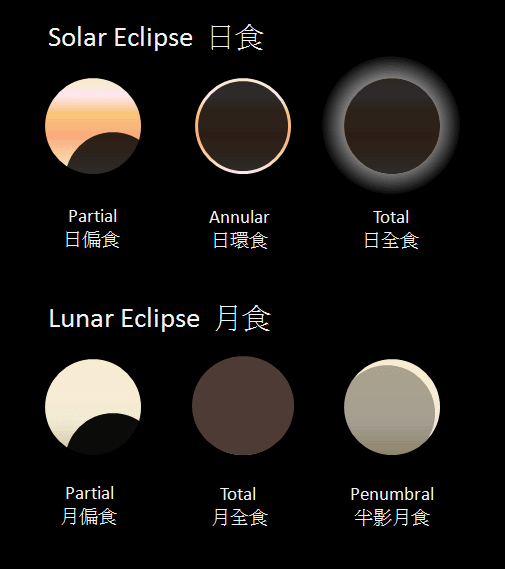
\includegraphics[width=0.5\linewidth]{images/ecltype.png}
    \caption{日月食的种类和图像}
    \label{fig:eclipse}
\end{figure}

本文工作的核心目标是通过建立包含太阳、地球、月球及木星的四体动力学模型,结合四阶龙格-库塔(Runge-Kutta)数值积分方法,实现未来50年内日月食事件类型与发生时刻的高精度预测。选择四阶龙格-库塔方法,源于其对微分方程初值问题的高精度求解特性——该方法通过多步加权平均策略有效抑制局部截断误差,在保证计算稳定性的同时,能够适应地月系轨道长期演化中摄动力引起的非线性效应。在太阳系(见图\ref{})这一复杂引力系统中,太阳作为中心天体占据总质量的99.86\%,而行星际引力作用通过轨道共振与长期摄动深刻影响着各天体的运动轨迹。尽管传统日月食预测模型通常将太阳、地球、月球视为孤立三体系统,但本课题通过第二部分理论分析中的误差量化研究发现:若忽略木星这一太阳系最大行星(质量占行星总质量的60\%)的引力作用,在50年时间尺度上,地月轨道半长轴将产生约$10^{-4}AU$量级的系统性偏移,其累积效应足以导致日月食时刻预测出现分钟级偏差。这种偏差源于木星虽距离地月系约$4.2-6.2$AU,但其$1.9×10^{27}$kg的巨大质量通过引力势的二阶项对地月轨道产生周期性摄动,其影响强度经计算可达$10^{-5}$量级(见\ref{object_error}对象误差)。因此,构建包含木星的四体模型是还原太阳系真实动力学图景的必要举措.
\begin{figure}[htbp]
    \centering
    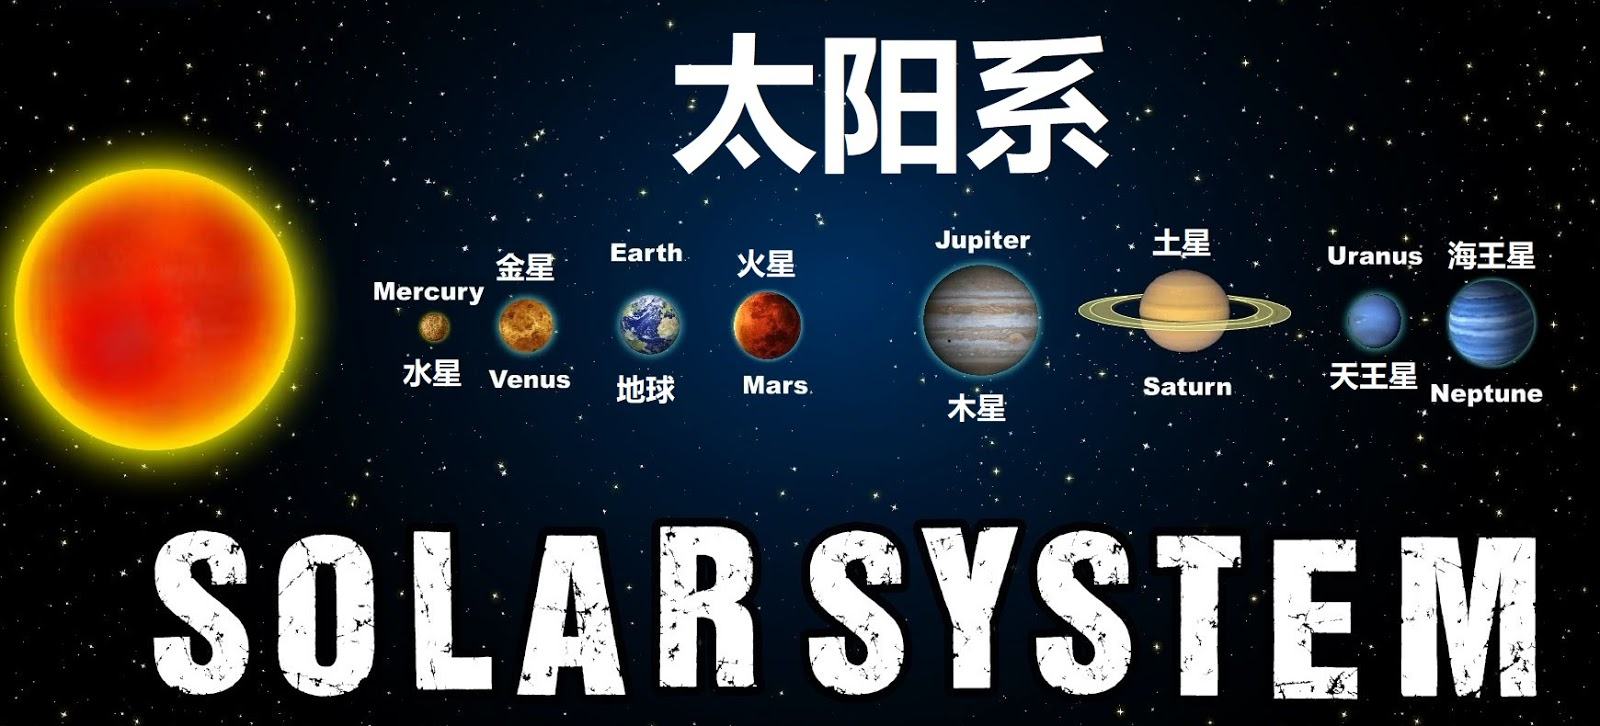
\includegraphics[width=0.5\linewidth]{images/太阳系.jpg}
    \caption{太阳系图片展示}
    \label{fig:solar system}
\end{figure}

本研究的创新性体现在两方面:其一,通过引入四阶龙格-库塔方法处理四体问题,突破了传统三体模型的局限性;其二,在判别条件设计中,我们严格依据国际天文联合会(IAU)的日月食判据标准,并针对数值计算结果开发了自动化事件检测算法。最终实现的预测结果与NASA权威星历表的高度吻合,不仅验证了模型的有效性,更彰显了数学建模在现代天体力学研究中的核心价值。
\section{理论分析}
\subsection{总论}
经典的$N$体运动方程为:
$$
M_i\ddot{\mathbf{r}}_i = \sum_{j=1}^N\frac{GM_iM_j}{||\mathbf{r}_j-\mathbf{r}_i||^3}(\mathbf{r}_j-\mathbf{r}_i)
$$
其中${M_i}$为各个天体的质量,$\mathbf{r}_i$为各个天体的位矢。
在模拟太阳系的过程中,完整的牛顿运动方程就应该是包含所有天体及其相互作用的N体运动。
\subsection{A Toy Model}
仅考虑三体运动,日地月系统的运动方程为:
\begin{align*}
    M_s\ddot{\mathbf{r}}_s&=\frac{GM_sM_e}{||\mathbf{r}_e||^3}\mathbf{r}_e+\frac{GM_sM_m}{||\mathbf{r}_m||^3}\mathbf{r}_m\\
    M_e\ddot{\mathbf{r}}_e&=-\frac{GM_sM_e}{||\mathbf{r}_e||^3}\mathbf{r}_e+\frac{GM_mM_e}{||\mathbf{r}_m-\mathbf{r}_e||^3}(\mathbf{r}_m-\mathbf{r}_e)\\
    M_m\ddot{\mathbf{r}}_m&=-\frac{GM_sM_m}{||\mathbf{r}_m||^3}\mathbf{r}_m+\frac{GM_eM_m}{||\mathbf{r}_e-\mathbf{r}_m||^3}(\mathbf{r}_e-\mathbf{r}_m)
\end{align*}
\subsection{误差及修正分析}
本节中对常见的需要纳入考量的影响因素的误差及其处理方式做了讨论。
\subsubsection{理论误差}
这里主要讨论了使用的物理理论并非精确带来的误差。
\paragraph{相对论}
狭义及广义相对论直接改变了最底层运动方程,其带来的影响无法严格计算,但影响的量级可以估计为 $\epsilon_r=(\frac{v}{c})^2\sim(\frac{2\pi r_e}{cT_e})^2\sim1\times10^{-8}$。
\\
\\
相对论(尤其是广义相对论)的引入会极大地增加求解的难度和复杂度,在这里不得不将其忽略,因此所得结果的误差界量级至少也有$10^{-8}$,此后所有影响量级在此之下的误差均会在讨论中指出并直接忽略。
\subsubsection{对象误差}
这里主要讨论了讨论的日地月系统外的天体系统及其效应带来的误差。
\paragraph{大行星和惯性力}
以木星为代表的大行星质量相对大,与地球距离相对近,其产生的引力扰动量级可以估计为$\epsilon_j\sim\frac{M_jr_e^2}{M_s(r_j-r_e)^2}\sim5\times10^{-5}$。
同时,太阳受到太阳系内各个行星的作用导致以太阳作为参考系时天体受到惯性力的作用,其产生的扰动量级可以估计为$\epsilon_a\sim\frac{M_jr_e^2}{M_sr_j^2}\sim4\times10^{-5}$,这个扰动与大行星的扰动同源,必须同时忽略或纳入考虑。
\paragraph{银河系以及更大的天体系统}
太阳系以约2.2亿个地球年为周期绕银河系作半径约为2.6万光年公转,同时银河系的其他部分的引力也会对太阳系中的天体产生长程作用,这个作用的强度可利用潮汐效应来估计$\epsilon_g\sim(\frac{2\pi}{T_s})^2r_s\frac{r_e}{r_{nearest}}\sim8\times10^{-16}$,可以直接忽略。
\label{object_error}
\\
\\
为处理大行星和惯性力带来的影响,除了直接将大行星加入天体系统进行模拟,也可以采用渐进微扰的思路。
将各个系统绕太阳作独立圆周运动作为零阶微扰的结果,各个系统间的影响视作一阶效应,由于二阶及更高的效应量级为$\epsilon^2\sim10^{-10}$可以忽略,我们最终求解的系统就是一个独立系统加上其他部分对其一阶微扰的结果。
处理一个N体问题的复杂度为$O(N^2)$,而将大行星的影响以微扰的形式加入的计算复杂度为$O(N)$。
因此当$N$足够大时,这个方案能极大的简化模拟,然而在实际应用中发现唯二对系统产生有效影响的行星只有木星和金星,在这个系统尺度下微扰的方法并没有优势。
\subsubsection{几何误差}
这里主要讨论将天体建模为质点带来的引力计算上的误差。
\paragraph{非球形建模}众所周知由于自转效应的影响地球是一个两极稍扁赤道略鼓的椭球,这就导致地球的引力并非严格等效于球心处的质点,考虑引力场的的球谐展开:
\begin{align*}
    G(\mathbf{r})&=\int_{\Omega}\frac{G\rho(\mathbf{R})}{||\mathbf{R}-\mathbf{r}||}\mathrm{d}^3\mathbf{R}\\
    &=G\sum_{n=0}^\infty\frac{1}{r^{n+1}}\int_\Omega R^n\rho(\mathbf{R})P_n(\cos{\psi})\mathrm{d}^3\mathbf{R}
\end{align*}
其中$P_n$为$n$阶勒让德多项式。
可见高阶矩的影响随着距离的增加而迅速减弱(以地月系统为例$\frac{||\mathbf{R}_e||}{||\mathbf{r}_m-\mathbf{r}_e||}\sim0.02$),实验测量给出地球二阶系数的量级$J_2\sim1\times10^{-3}$,因此唯一可能有有效影响的$J_2$摄动在地月系统中影响量级为$\epsilon_e\sim(\frac{||\mathbf{R}_e||}{||\mathbf{r}_m-\mathbf{r}_e||})^2J_2\sim4\times10^{-7}$,而与太阳相关的摄动影响更加不明显,无需纳入考虑。
\subsubsection{观测误差}
由于我们预测的是“观测到日(月)食的时间”,所以一些观测建模上的误差也要纳入讨论。
\paragraph{光传播用时}
在宇宙尺度中光速会让日(月)食的发生不再是一个单纯的几何问题,由于发生时日地月基本在一条直线上,月(地)对太阳光线的遮挡与地球上观测到这个现象之间间隔的时间可以直接用光传播的时间进行近似$\Delta t_l\sim2\frac{||\mathbf{r}_e-\mathbf{r}_m||}{c}\sim2s$,发生和观测时间的不同步也会对日(月)食判断的几何条件带来影响,这个影响带来的时间上的误差也在同一量级。
\paragraph{大气}
标准大气的折射率$n_a=1+2.9\times10^{-4}$,在地球大气层随着高度的上升,这个值由于空气变得稀薄越来越接近于1,这会导致光线产生弯曲。另外,光的散射也会导致部分波长的光到达月球后强度有不同程度的减弱,从而带来其他观测上的效应。对于日食,这个偏转作用在地球表面量级为$\theta=\theta_0-\sin^{-1}(\frac{1}{n_a}\sin\theta_0)\sim1.4^\circ$,对时间的影响量级为$\Delta t_n\sim\frac{\theta}{2\pi}T_0\sim20s$,但是这个误差随一天不同时间的变化明显,在接近日出(日落)时最为明显,在正午则无理论影响。对于月食,这个误差等效为地球半径的变化(即大气层的一部分由于光的被散射或是吸收从而增大了地球的阴影范围),但因为大气密度随着海拔指数的下降,在距离地表50km处就下降到地表处的1\%以下,大气对地球有效半径的影响甚至没有地球本身形状带来的影响明显。
\paragraph{其他几何因素}
地月半径的不均匀等其他几何因素也会对日(月)食的形态产生影响,但不会显式的影响到日(月)食发生的客观时间。
\\
\\
这一部分出现的误差由于直接作用于观测端,并不能直接与前面提到的建模误差进行量级上的比较。可以根据最后误差的敏感性来考量是否将其纳入考虑。
\subsubsection{结论}
按照前面提出的处理方法,最终观测时间的误差阶为$4\times10^{-7}\pm20s$。
在50年的尺度下看,也就是$\pm50 y.\times 4\times10^{-7}\pm20 s\sim \pm10min$。
以上分析均为理论估计,具体的影响量级需要在之后的实验中做进一步验证。
\subsection{运动方程的无量纲化处理}
为了避免大量的不同量级常数运算,在数值模拟过程中对所有运动方程做了无量纲化处理。
具体为:
\begin{align*}
    \tilde{t}&=\frac{t}{3600s/h}\\
    \tilde{r}&=\frac{r}{1.495979\times10^8km/a.u.}
\end{align*}
同时修改质量的量纲,使得万有引力常数$G=1$。
\section{数值算法}

\section{实验结果}
目前根据我们的数值算法,已实现对2025年至2075年全部日食和月食事件的百分百预测,其中对食分时刻的预测误差控制在30min以内,极少事件会出现20min以上的误差(见图\ref{fig:eclipse_error})

\begin{figure}[h]
    \centering
    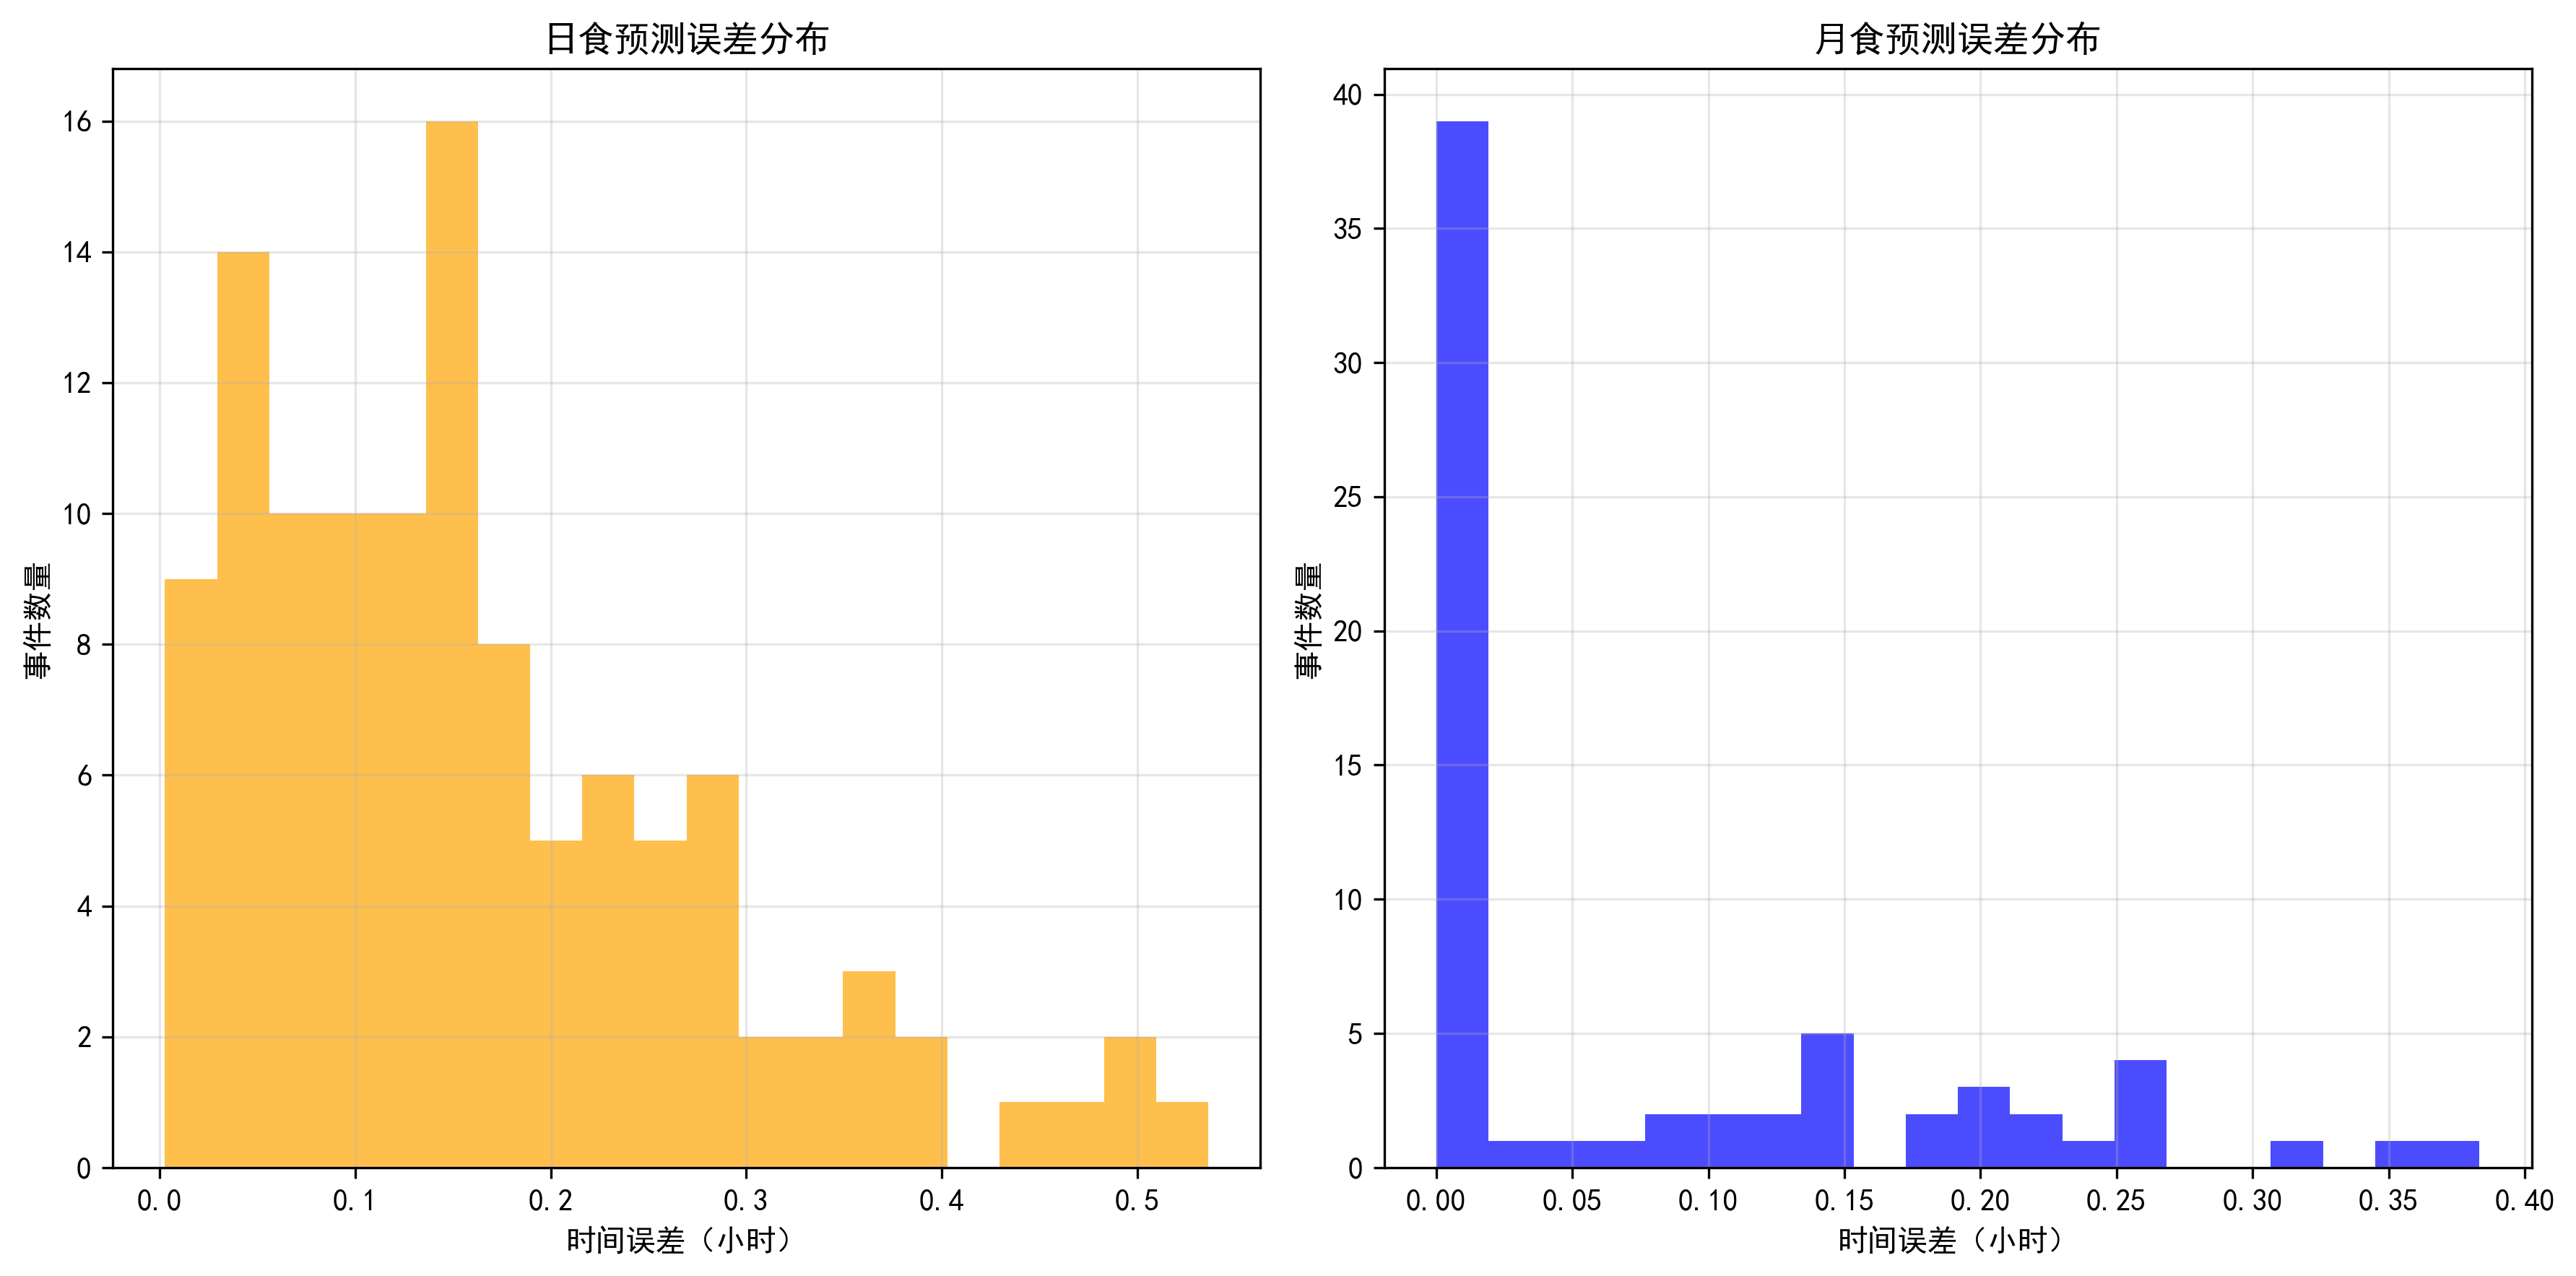
\includegraphics[width=0.5\linewidth]{images/error_distribution.png}
    \caption{2025年至2075年日食和月食预测事件食甚时刻的误差分布}
    \label{fig:eclipse_error}
\end{figure}
\section{讨论}

\section{附录}

\end{document}
